\documentclass{article}
\usepackage[utf8]{inputenc}
\usepackage{graphicx}
\usepackage{listings}
\usepackage{color}
\usepackage{fixltx2e}

\def\infinity{\rotatebox{90}{8}}
\definecolor{dkgreen}{rgb}{0,0.6,0}
\definecolor{gray}{rgb}{0.5,0.5,0.5}
\definecolor{mauve}{rgb}{0.58,0,0.82}

\lstset{language=C,
  numbers=left,
  stepnumber=1,    
  firstnumber=1,
  numberfirstline=true
  aboveskip=5mm,
  belowskip=5mm,
  showstringspaces=false,
  columns=flexible,
  basicstyle={\small\ttfamily},
  numberstyle=\tiny\color{gray},
  keywordstyle=\color{blue},
  commentstyle=\color{dkgreen},
  stringstyle=\color{mauve},
  breaklines=true,
  breakatwhitespace=true
  tabsize=3
}

\title{Artificial Intelligence 1 - Lab 4}
\author{Guilherme Alles (s2847264) \& Isadora Possebon (s2847302)} 

\begin{document}

\maketitle

\section*{Theory}
\subsection*{Exercise 1 - Eight Queens Problem}
\subsubsection*{1)}
\paragraph{} The variables on this problem are N0, N1, N2, N3, N4, N5, N6 and N7. Each variable has a domain containing the numbers from 1 to 8. We can consider that each variable N\textsubscript{i} represents one column on the problem, and the value assigned to the variable represents the position (row) of the queen on each column.

\subsubsection*{2)}
\paragraph{Constraints} There must not be more than one queen in every row or diagonal of the board. Because the formulation of the problem assumes that every queen is already in a different column, we do not need to add this constraint. With the notation used in the applet, the constraints would look like this:

\[\forall N\textsubscript{i}, N\textsubscript{j}\]
\[N\textsubscript{i} \neq N\textsubscript{j} \land\]
\[\mid i - j\mid  \neq  \mid N\textsubscript{i} - N\textsubscript{j}\mid\]

\subsubsection*{3)}
\paragraph{Random Walk} The random walk algorithm did not find an answer in less than 100 steps. Because the algorithm chooses randomly what will be the next step to take (which variable to assign), there is no guarantee that it will find a solution at all. In fact, increasing the number of maximum steps to 1000 also did not generate a solution.

\paragraph{Greedy Descent} By simply choosing a state that decreases the evaluation function of the problem, the greedy descent algorithm usually finds a solution. However, the completion of the algorithm is not guaranteed. In some cases, the algorithm can get stuck at local minimas or present a behaviour similar to the hill descending with the Rosenbrock function (where the evaluation decreases in such a slowly pace that it does not yield a solution in practical time). Although this algorithm is not 100\% reliable, this was the one that generated solutions faster. In our tests, it was not rare to obtain a solution to the problem in less than 20 steps.

\paragraph{Greedy Descent with min conflicts heuristic} This method randomly chooses a variable to assign a value, and then chooses the value which generates less conflicts to be assigned. This approach usually solves the problem relatively fast (in less than 100 steps), but is still susceptible to getting stuck at local minimas. Also, because it picks a random variable to assign a value, the exact same starting state may take different amounts of steps to solve when running multiple times.

\paragraph{Simulated Annealing} The simulated annealing algorithm works by allowing "bad" choices to be made with a certain probability (that depends on a function of time usually called \textit{temperature}). The "cooler" the temperature is, the less likely it is that the algorithm will take a bad choice. By making choices that does not specifically generate a better state, we can avoid local minimas and eventually get to a solution. In theory, we can achieve 100\% success rate if we decrease the temperature slowly enough. The downside of simulated annealing is exactly that: we need to define parameters to which we decrease the temperature, and the success rate of the algorithm is directly related to this choice of parameters. The set of parameters shown below were able to find a solution to the Eight Queens Problem in 100\% of the times.
\begin{itemize}
\item Maximum number of steps: 10000;
\item Starting temperature: 1000 degrees;
\item Descent function: Logarithmic;
\item Descent rate: 1.0\%;
\item Maintain temperature for 10 attempts.
\end{itemize}
\paragraph{} Even though the simulated annealing algorithm has a very high success rate, it is not the fastest algorithm we tested. Finding a solution relies on slowly decreasing the temperature, which means we need a bigger number of steps to complete the task. If the main concern is reliability, though, this algorithm might be the best choice between the ones we tested.

\pagebreak

\paragraph{Solution} Here is one of the solutions generated by the applet.

\begin{figure}[!ht]
\centering
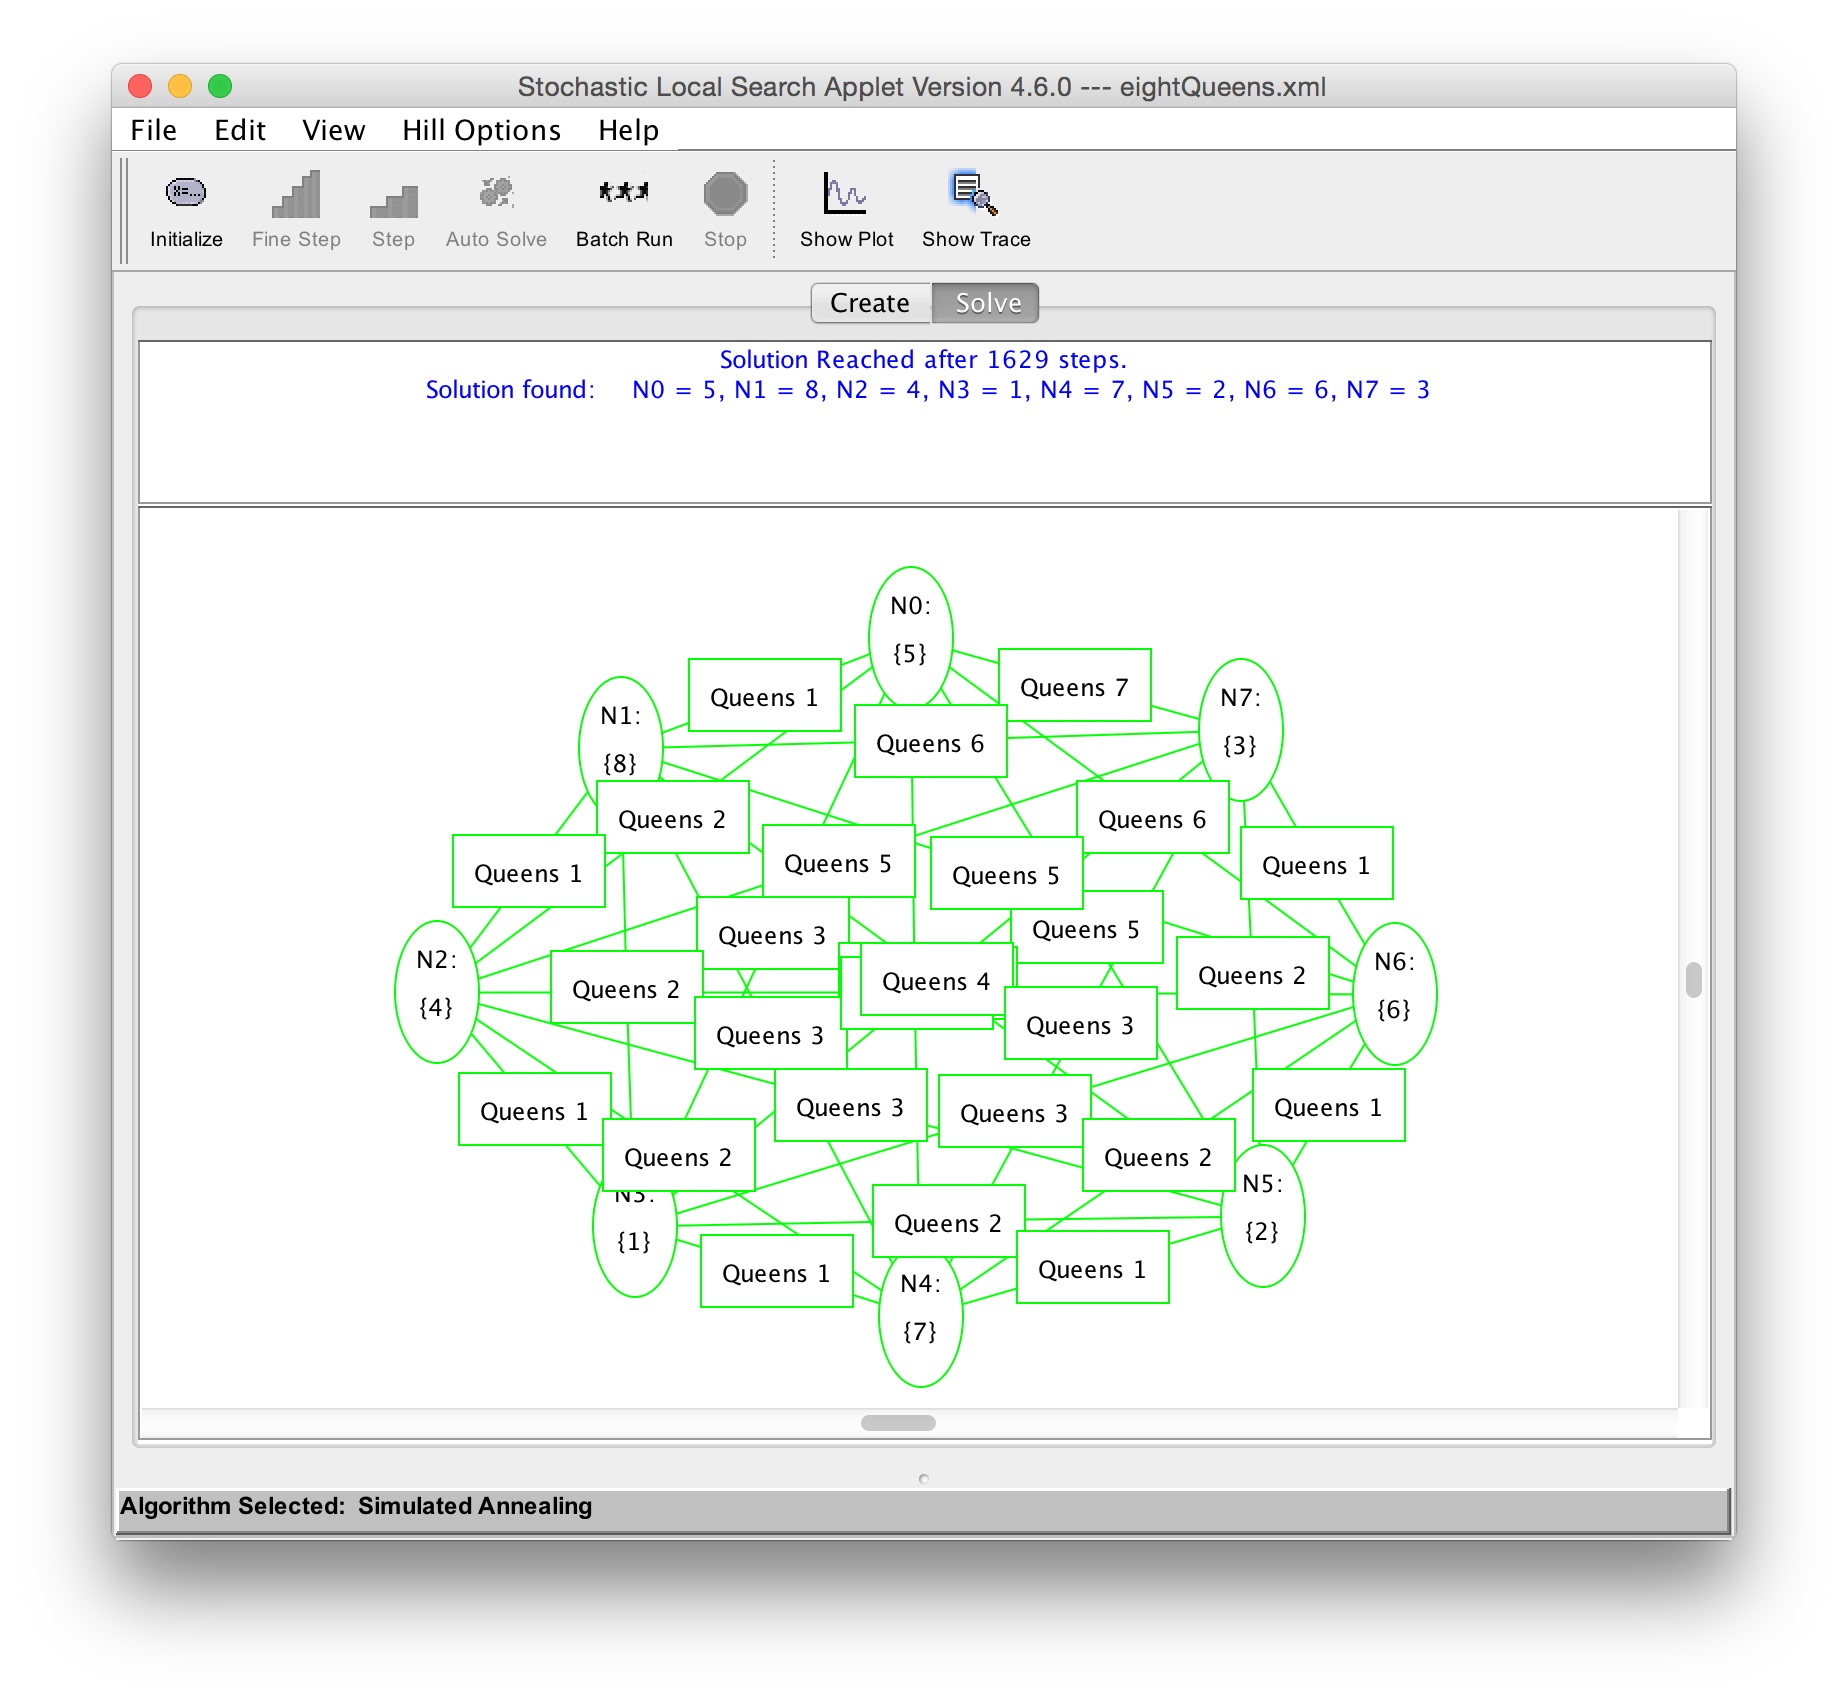
\includegraphics[width=0.8\textwidth]{SA-solution}
\caption{Solution generated using the simulated annealing algorithm}
\label{SA - solution}
\end{figure}


\subsection*{Exercise 2 - 4x4 sudoku}
\paragraph{} For rephrasing this problem as a standard CSP problem, we defined the variables as cells of the board, indicated by its position (for example, 1x3, 2x2, etc.). For simplification of the problem, the cell's domain is the set of possible choices, considering the values fixed on the board and the concept of constraint propagation, in order to reduce the problem size. The constraint is that values located on the same row, same column or same subset must be different. The image below shows the CSP graph.

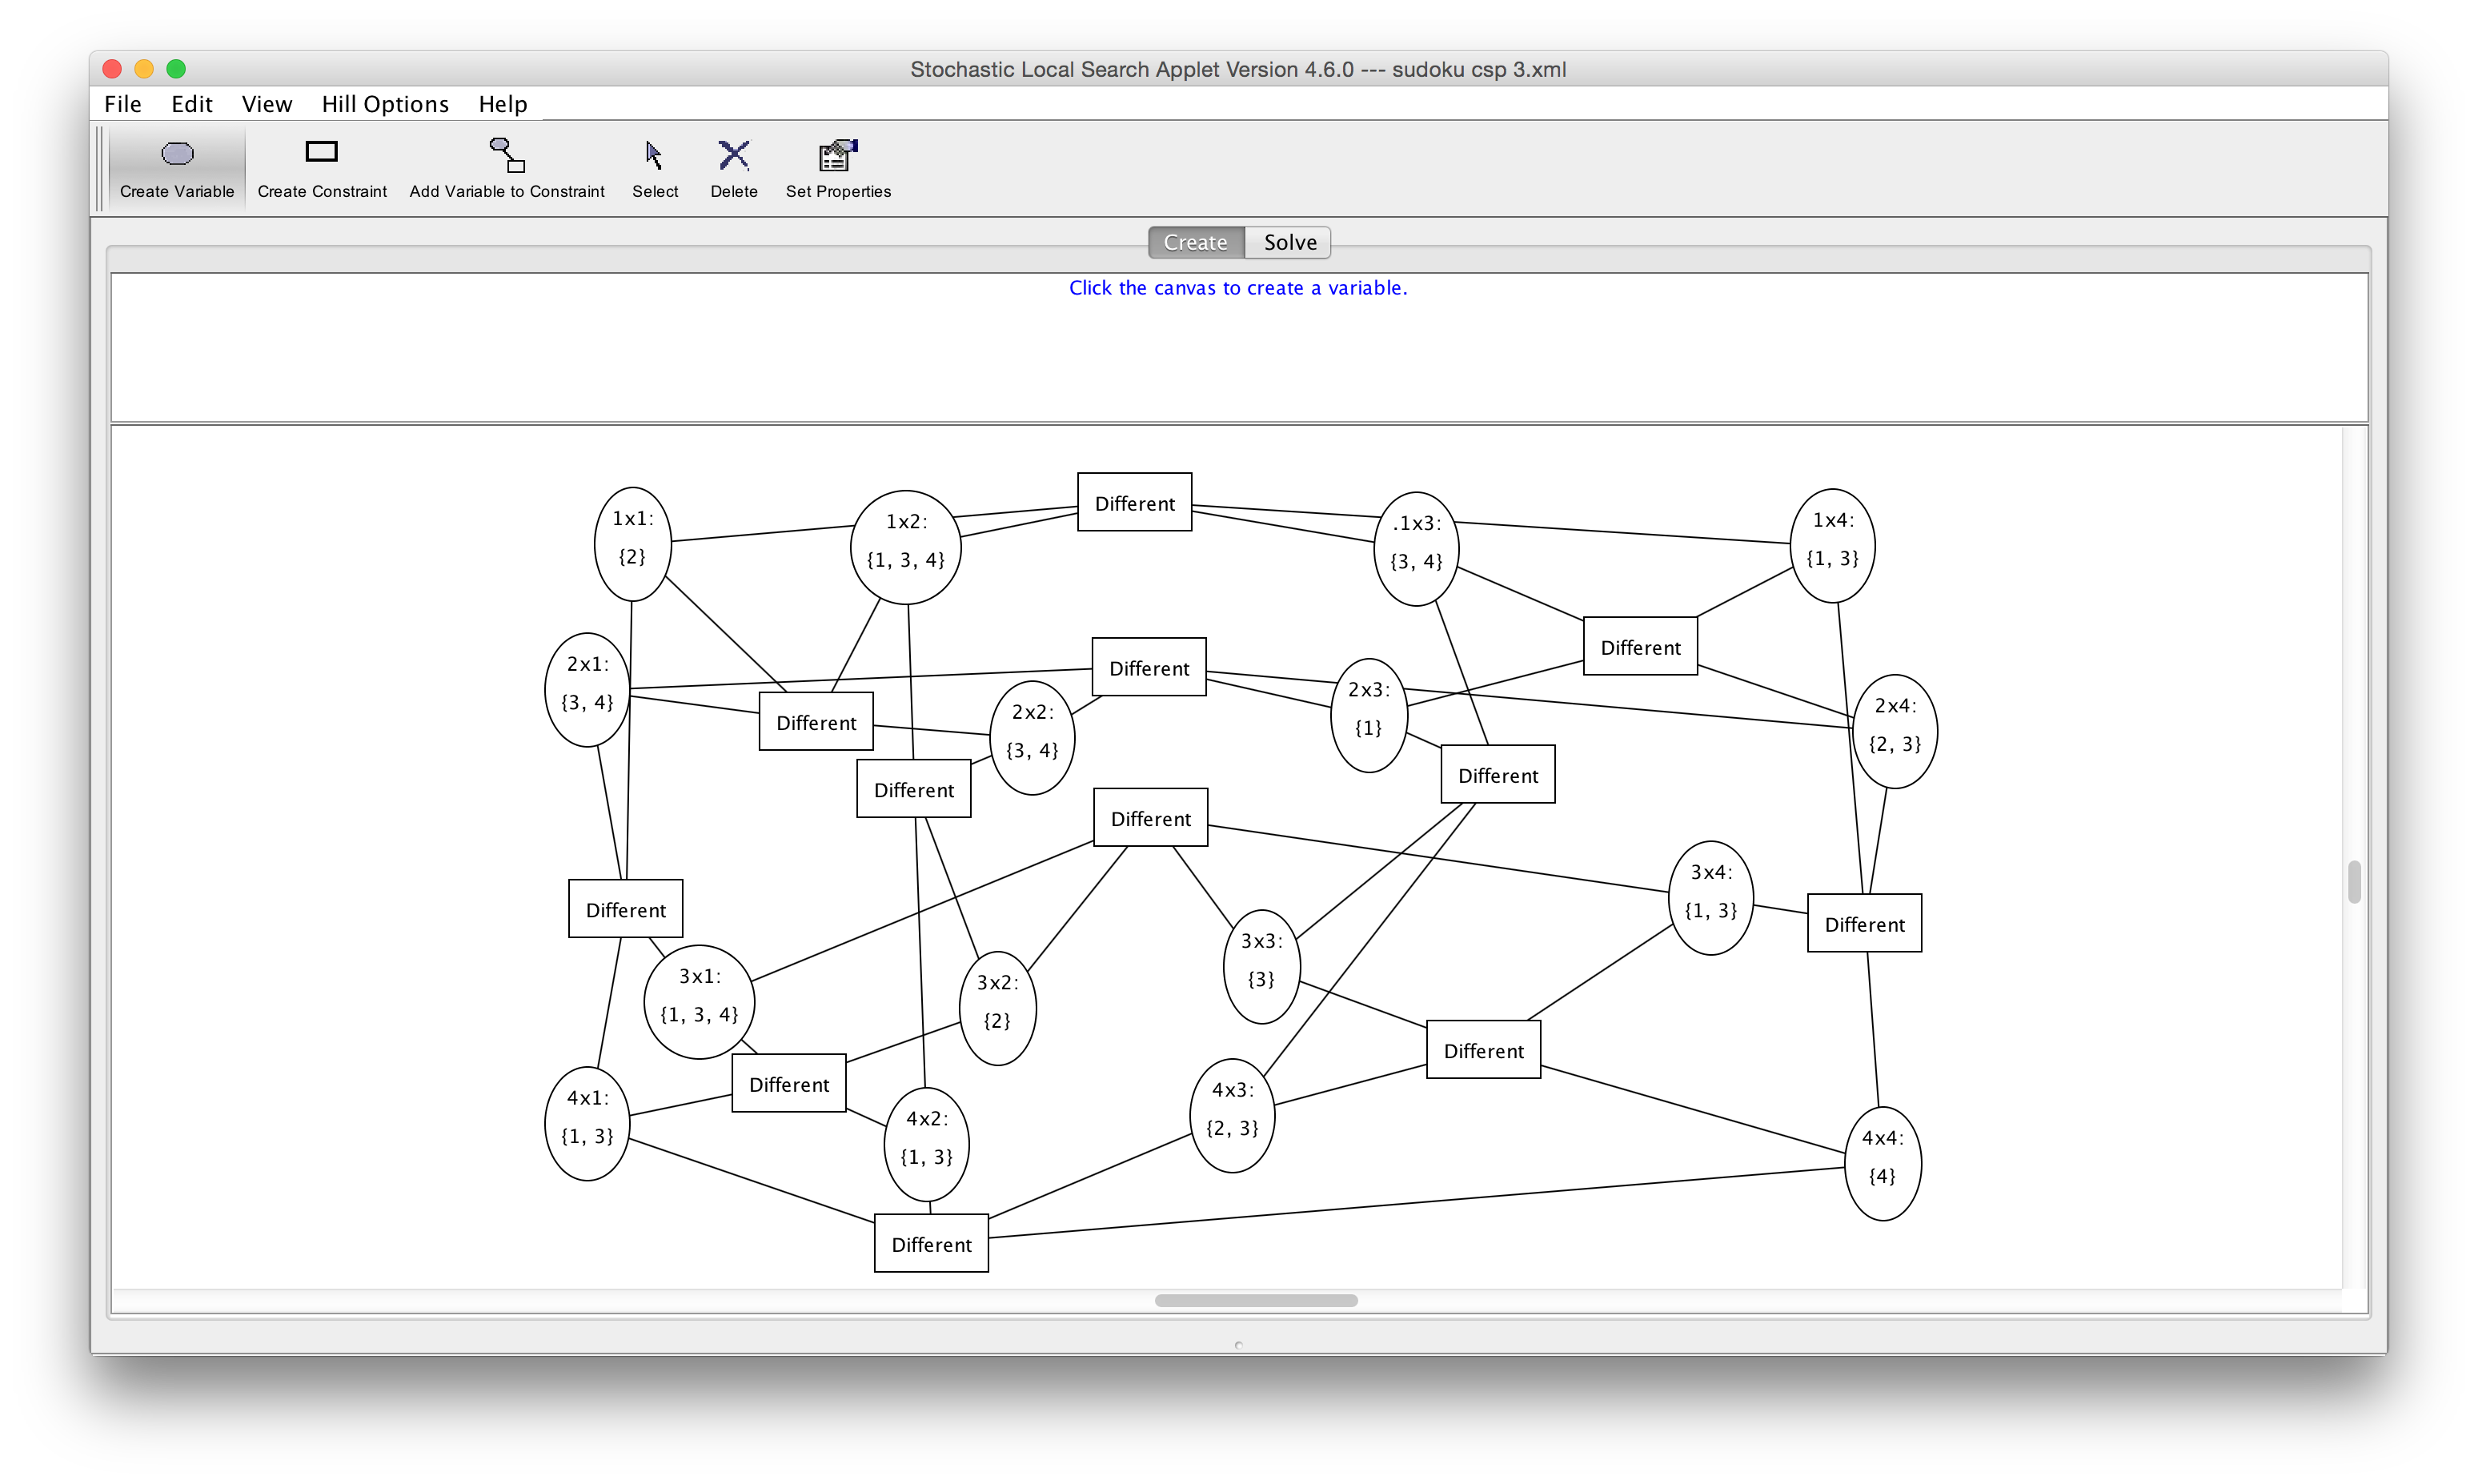
\includegraphics[width=\textwidth]{sudoku}

\paragraph{} Using the provided applet to solve this problem and by choosing the initial value as the lower value, we used all the available algorithms in order to see its performance. Greedy descent showed the best performance, taking 6 steps to find a solution. The same performance was seen with Greedy descent with random restart algorithm. The others algorithms, however, could not find a solution after 100 steps.
%%% Nao imagino porque só eles tenham funcionado.

\section*{Programming} 
%The programming part follows the same template used during ADinC and Imperative Programming
\subsection*{a)}
\paragraph{} Assuming optimal play, the two following trees tell us that whenever we reach \textit{k=2}, \textit{k=3} or \textit{k=4}, the player who plays next will win.

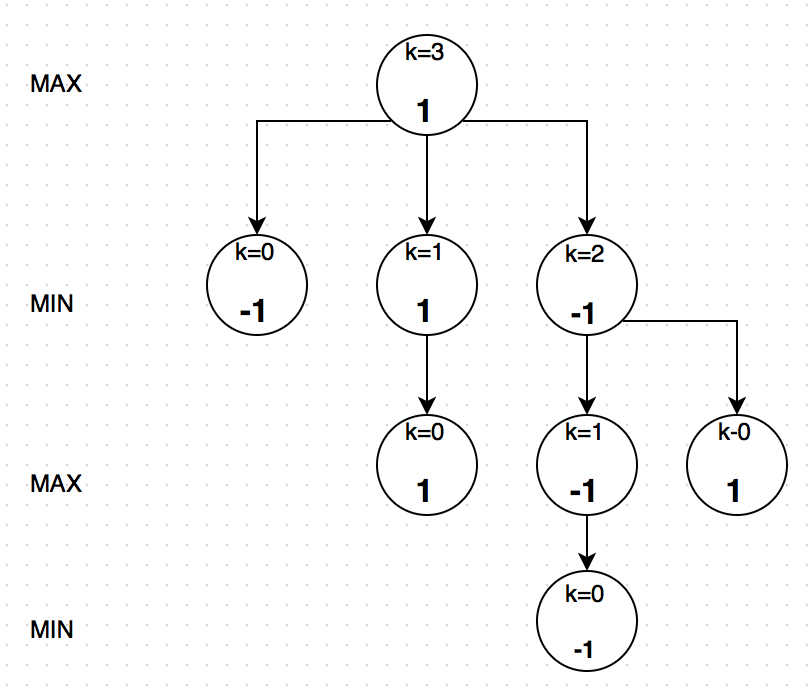
\includegraphics[width=\textwidth]{k=3}
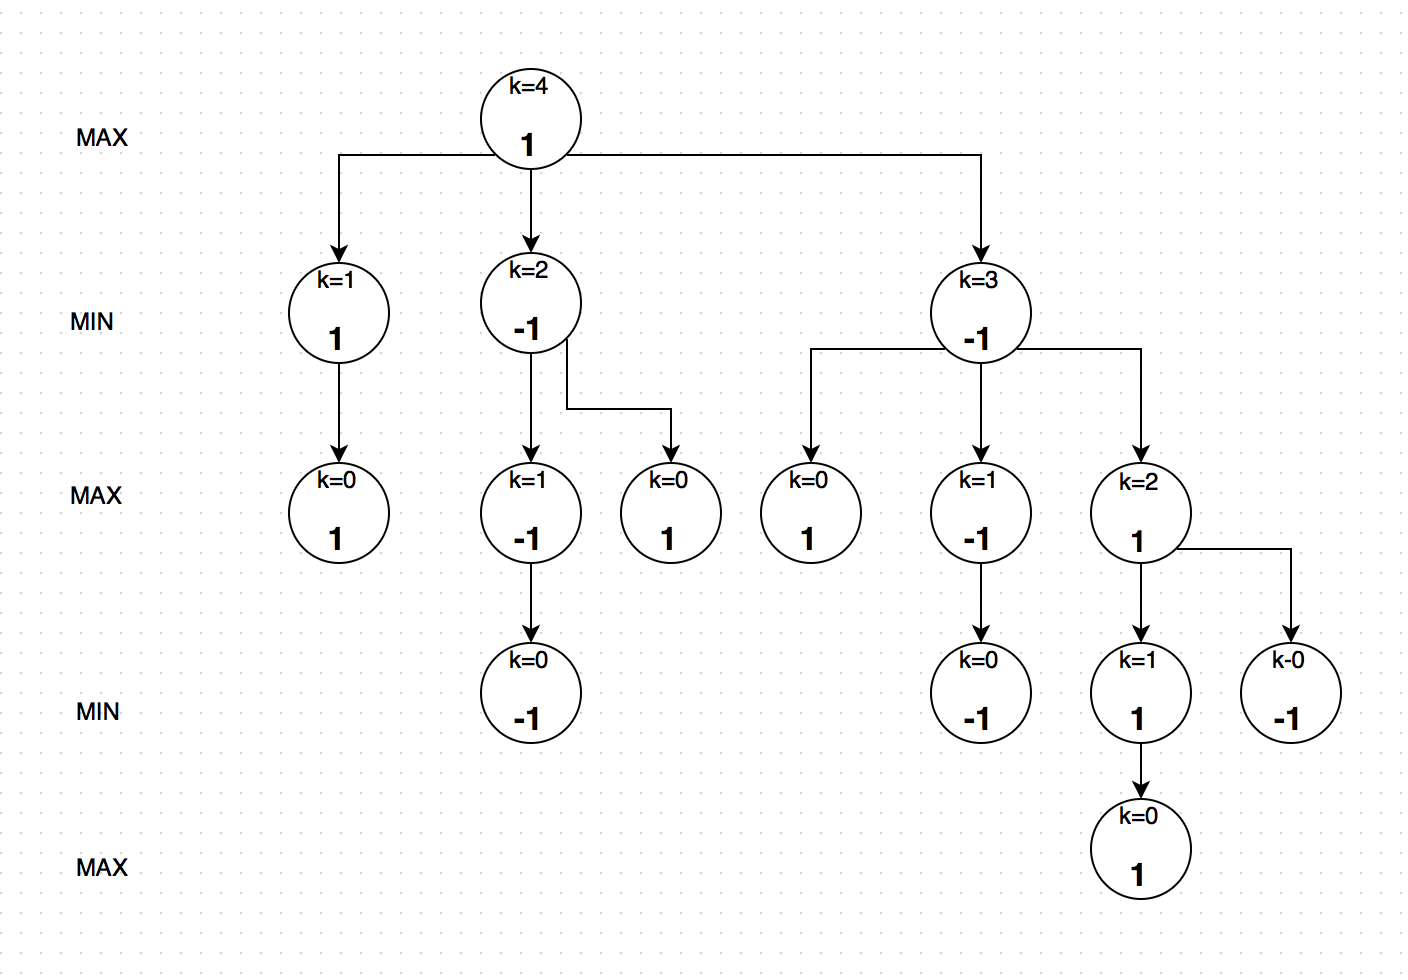
\includegraphics[width=\textwidth]{k=4}

\paragraph{} If we consider \textit{k=2}, \textit{k=3} or \textit{k=4} now as leaf nodes (assigning -1 or 1 according to the current player), we can derive the following for \textit{k=5} and \textit{k=6}:

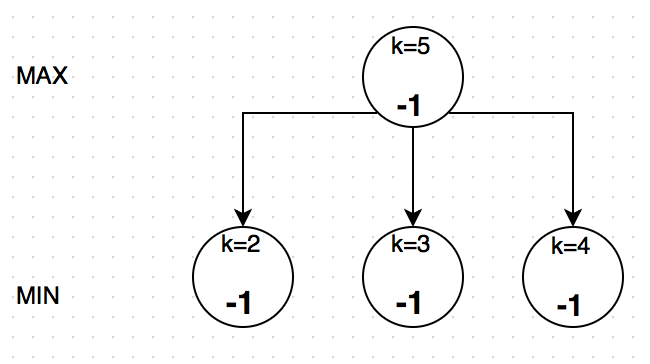
\includegraphics[width=\textwidth]{k=5}
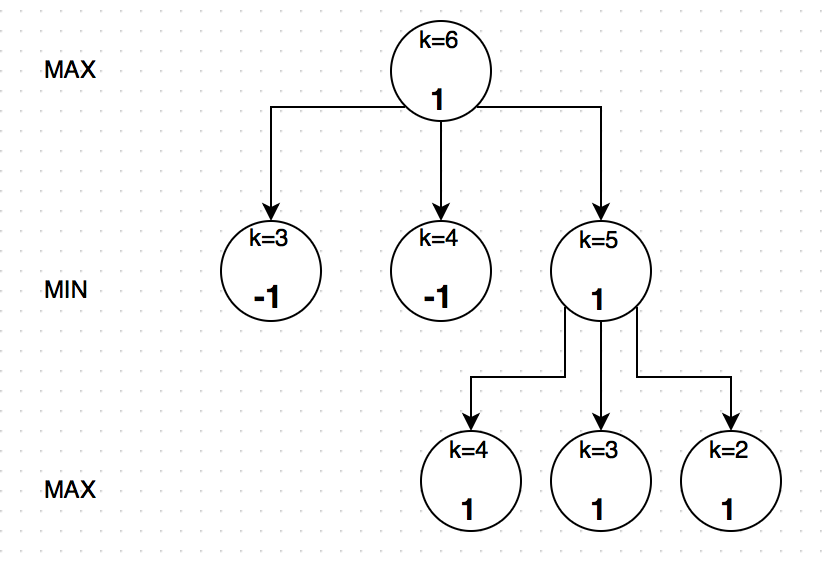
\includegraphics[width=\textwidth]{k=6}

\subsection*{c)}
If we run the program for the suggested values, it takes a long time to find a solution. For n = 40, for example, it is not feasible to find a solution in practical time. This happens because the tree is too big and the search takes a long time to find the best move.

\paragraph{}In order to solve this problem, we can use a transposition table. A transposition table is used to store nodes that were already generated, in order to speed up search. It contains keys and values corresponding to the keys, that is, a game state and search results associated with it. This technique is used in game development in order to make visiting repeated nodes more efficient.

\paragraph{}For this case, we created a transposition table with \textit{turn} and \textit{state} as keys, and the evaluation of the respective state as the value. Therefore, during the negamax evaluation, whenever the algorithm reaches a node that is already on the transposition table, we simply return the correspondent value. If the node is not on the transposition table, we evaluate it and add it to the table.

\paragraph{} As expected, this approach provides a significant speedup to the search and, therefore, enables the algorithm to find a solution for bigger numbers faster.

\subsection*{Program description}
The provided program simulates the game of Nim. This game consists of a pile of sticks and two players taking turns to remove sticks from the pile (with the constraint that a player can only remove 1, 2 or 3 sticks from the pile per turn). The last player to remove a stick from the pile loses.

\subsection*{Problem analysis}
The problem consisted of implementing the negamax algorithm, in order to avoid code replication (which existed with \textit{minValue()} and \textit{maxValue()}). Moreover, the algorithm should use a transposition table to be able to solve the game for a bigger number of sticks (from 3 to 100).

\subsection*{Program design}
We decided to maintain the original program design, only changing some values to constants (the definitions of INFINITY, MAX and MIN conflicted with the \textit{math.h} header). 

\subsection*{Program evaluation}
We could not implement the variation where the pair movement+value is returned after every recursion of the negamax algorithm. The other requirements were implemented and worked as expected.

\subsection*{Program output}
\begin{lstlisting}
Which algorithm to use? (Minimax = 0, Negamax = 1):
1
30: Max takes 1
29: Min takes 1
28: Max takes 3
25: Min takes 1
24: Max takes 3
21: Min takes 1
20: Max takes 3
17: Min takes 1
16: Max takes 3
13: Min takes 1
12: Max takes 3
9: Min takes 1
8: Max takes 3
5: Min takes 1
4: Max takes 3
1: Min looses

\end{lstlisting}

\subsection*{Source code}
\begin{lstlisting}
#include <stdio.h>
#include <stdlib.h>


#define MAX_V 0
#define MIN_V 1

#define MAX_STICKS 100
#define INF 9999999

int transposition_table[2][MAX_STICKS +1];

int minValue(int state); /* forward declaration: mutual recursion */

void addValueToTable(int turn, int state, int value)
{
    transposition_table[turn][state] = value;
}

int maxValue(int state) {
    int move, max = -INF;
    /* terminal state ? */
    if (state == 1) {
        return -1; /* Min wins if max is in a terminal state */
    }
    
    /* non-terminal state */
    for (move = 1; move <= 3; move++) {
        if (state - move > 0) { /* legal move */
            
            int m = minValue(state - move);
            if (m > max) max = m;
        }
    }
    return max;
}

int minValue(int state) {
    int move, min = INF;
    /* terminal state ? */
    if (state == 1) {
        return 1; /* Max wins if min is in a terminal state */
    }
    
    /* non-terminal state */
    for (move = 1; move <= 3; move++) {
        if (state - move > 0) { /* legal move */
            
            int m = maxValue(state - move);
            if (m < min) min = m;
        }
    }
    
    return min;
}

int minimaxDecision(int state, int turn) {
    int move, bestmove=0, max, min;
    if (turn == MAX_V) {
        max = -INF;
        for (move = 1; move <= 3; move++) {
            if (state - move > 0) { /* legal move */
                int m = minValue(state - move);
                if (m > max) {
                    max = m;
                    bestmove = move;
                }
            }
        }
        return bestmove;
    }
    /* turn == MIN */
    min = INF;
    for (move = 1; move <= 3; move++) {
        if (state - move > 0) { /* legal move */
            int m = maxValue(state - move);
            if (m < min) {
                min = m;
                bestmove = move;
            }
        }
    }
    return bestmove;
}

int negamaxValue(int state, int turn) {
    int move, max = -INF;
    
    /* terminal state ? */
    if (state == 1) {
        return -1;
    }
    /* non-terminal state */
    for (move = 1; move <= 3; move++) {
        if (state - move > 0) { /* legal move */
            
            if (transposition_table[turn][state-move] != -1)
            {
                return transposition_table[turn][state-move];
            }
            int m =  - negamaxValue(state - move, 1 - turn);
            if (m > max) {
                addValueToTable(turn, state - move, m);
                max = m;
            }
        }
    }
    return max;
}

int negamaxDecision(int state, int turn) {
    int move, bestmove = 0, max = -INF;
   
    for (move=1; move<=3; move++) {
        if (state - move > 0) {
            int m = -negamaxValue(state - move, 1 - turn);
            if (m > max) {
                max = m;
                bestmove = move;
            }
        }
    }
    return bestmove;
}


void playNim(int state) {
    int turn = 0;
    while (state != 1) {
        int action = minimaxDecision(state, turn);
        printf("\%d: \%s takes \%d\n", state, (turn==MAX_V ? "Max" : "Min"), action);
        state = state - action;
        turn = 1 - turn;
    }
    printf("1: \%s looses\n", (turn==MAX_V ? "Max" : "Min"));
}

void playNimNegamax(int state)
{
    int turn = 0;
    while (state != 1)
    {
        int action = negamaxDecision(state, turn);
        printf("\%d: \%s takes \%d\n", state, (turn==MAX_V ? "Max" : "Min"), action);
        state = state - action;
        turn = 1 - turn;
    }
    printf("1: \%s looses\n", (turn==MAX_V ? "Max" : "Min"));
}


void initializeTranspositionTable()
{
    // Initializes all movements with -1.
    for (int i = 0; i <= MAX_STICKS; i++)
    {
        transposition_table[0][i] = -1;
        transposition_table[1][i] = -1;
    }
}

int main(int argc, char *argv[]) {
    if ((argc != 2) || (atoi(argv[1]) < 3)) {
        fprintf(stderr, "Usage: \%s <number of sticks>, where ", argv[0]);
        fprintf(stderr, "<number of sticks> must be at least 3!\n");
        return -1;
    }
    
    initializeTranspositionTable();
    
    int option = -1;
    while (!(option == 0 || option == 1)) {
        printf("Which algorithm to use? (Minimax = 0, Negamax = 1):\n");
        scanf("\%d", &option);
    }
    switch (option) {
        case 0:
            playNim(atoi(argv[1]));
            break;
        case 1:
            playNimNegamax(atoi(argv[1]));
            break;
        default:
            playNim(atoi(argv[1]));
            break;
    }
    
    return 0;
}

\end{lstlisting}
\end{document}